\section{Lektion 22-02-2018}

\begin{enumerate}
	\item Virtuel Akustik
	\item Ray Tracing Method
	\item Image Source Method
	\item Reflektogram
\end{enumerate}

\noindent\fbox{\parbox{\textwidth}{
		\begin{itemize}
		\item \textbf{Pensum:} 
		\begin{enumerate}
			\item The Use of Computer Modeling in Room Acoustics, \\J. H. Rindel
			\item Image Method For Efficiently Simulating Small-Room\\ Acoustics, Jont B. Allen and David A. Berkley
		\end{enumerate}
		\item \textbf{Opgaver:} 
		\begin{enumerate}
			\item Lyd og Akustik - Lektion 5 - opgaver og øvelser
		\end{enumerate}
	\end{itemize}
}} \vspace{3mm}

\subsection{Virtuel Akustik}
\begin{itemize}
	\item Audio for virtual reality har mange termer såsom auralization, virtual acoustics, binaural room simulation  og auditory display.
	\item Auralization er en two-stage proces:
	\begin{itemize}
		\item Udregning af impulsrespons (IR) for et akustisk rum.
		\item Convolution af impulsresponset med et tørt (anechoically
		recorded eller syntetisk genereret) signal.
	\end{itemize} 
\end{itemize}

\subsection{Ray Tracing Method}
\begin{itemize}
	\item Den samlede energi der udsendes af en source er fordelt som stråler i et bestemt antal af retninger.
	\item Energien af hver enkel stråle er lig med den samlede energi delt med antallet stråler. 
	\item Afhængig af overfladens absorption vil hver stråle spejles med indfaldsvinklen er lig med vinklen på refleksionen eller diffus reflekteret, hvor retningen af den reflekterede stråle er randomiseret.
	\item For at opnå et beregningsresultat relateret til en bestemt
	receiver position \textit{R1} er det nødvendigt at definere et område eller en volumen omkring receiveren for at fange strålerne.
	\item Der er en risiko for beregne falske refleksioner og at nogle mulige refleksioner ikke findes.
\end{itemize}

\begin{figure} [H]
	\centering
	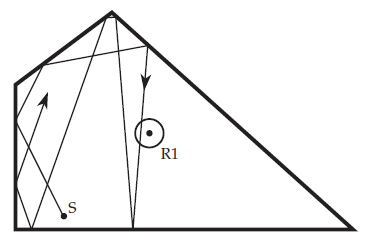
\includegraphics[width=.6\linewidth]{graphics/17.png}
	\caption{Ray Tracing - source S, receiver area R1.}
	\label{fig:17}
\end{figure}

\subsection{Image Source Method}
\begin{itemize}
	\item Et virtuelt image af den faktiske kilde (real source) bestemmes ved at reflektere kilden vinkelret på tværs af en rumgrænse (boundary).
	\item Den virtuelle kilde (image source) er placeret i en afstand \textit{d} der svarer til den dobbelte afstand mellem source og rumgrænsen (vinkelret).
	\item Afstanden mellem den virtuelle kilde S1 og receiveren R1 svarer til refleksions distancen (reflection path) mellem S og R1.
	\item Refleksionerne af alle reelle og virtuelle kilder, der krydser en rumgrænse, skaber et mirror image.
	\item Ved et rektangulært rum vil alle virtuelle kilder være synlige i alle positioner i rummet og beregningen er hurtig.
	\item Gælder ikke ved irregulære rum. Validering af hvert image er påkrævet og antallet af beregninger bliver hurtigt mange.
	\item 2. ordens refleksion når en stråle rammer 2 rumgrænser inden den når receiveren.
\end{itemize}

\begin{figure} [H]
	\centering
	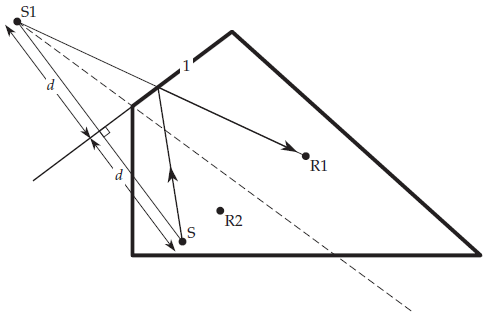
\includegraphics[width=.75\linewidth]{graphics/18.png}
	\caption{ISM - real source S, virtual source S1, receiver R1.}
	\label{fig:18}
\end{figure}

\noindent Estimat af antallet \textit{N} refleksioner som receiveren vil modtage indenfor tiden \textit{t}.

\begin{equation}
N_{refl}=\dfrac{4\pi c^3}{3V}t^3
\end{equation}

\noindent Ved \textit{n} antal rumgrænser = \textit{n} antal mulige 1. ordens image sources som kan medføre \textit{n-1} 2. ordens image sources. \\

\noindent Estimat af mulige image sources ved \textit{i} ordens image source. 

\begin{equation}
N_{sou}=1+\dfrac{n}{(n-2)}((n-1)^i -1)\approx (n-1)^i
\end{equation}

\newpage
\subsection{Reflektogram}
\begin{itemize}
	\item Viser ankomsten af tidlige refleksioner til en receiver.
	\item Arrival time (\textit{x-aksen}) og energi af refleksionen (\textit{y-aksen}).
\end{itemize}

\begin{figure} [H]
	\centering
	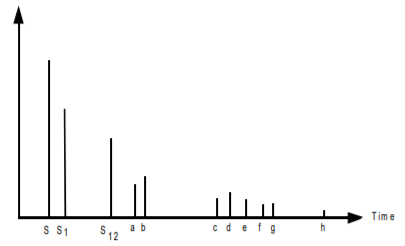
\includegraphics[width=.75\linewidth]{graphics/19.png}
	\caption{Reflectogram for receiver R med 2 image sources.}
	\label{fig:19}
\end{figure}

